
\documentclass[11pt,fleqn]{article} 
\usepackage[margin=0.8in, head=0.8in]{geometry} 
\usepackage{amsmath, amssymb, amsthm}
\usepackage{fancyhdr} 
\usepackage{palatino, url, multicol}
\usepackage{graphicx, pgfplots} 
\usepackage[all]{xy}
\usepackage{polynom} 
%\usepackage{pdfsync} %% I don't know why this messes up tabular column widths
\usepackage{enumerate}
\usepackage{framed}
\usepackage{setspace}
\usepackage{array,tikz}

\pgfplotsset{compat=1.6}

\pgfplotsset{soldot/.style={color=black,only marks,mark=*}} \pgfplotsset{holdot/.style={color=black,fill=white,only marks,mark=*}}
\pgfplotsset{my style/.append style={axis x line=middle, axis y line=
middle, xlabel={$x$}, ylabel={$y$} }}

%axis equal 
\pagestyle{fancy} 
\lfoot{}
\rfoot{3-8 Implicit Differentiation}

\begin{document}
\renewcommand{\headrulewidth}{0pt}
\newcommand{\blank}[1]{\rule{#1}{0.75pt}}
\newcommand{\bc}{\begin{center}}
\newcommand{\ec}{\end{center}}
\renewcommand{\d}{\displaystyle}

\vspace*{-0.7in}

%%%%%%%%%intro page
\begin{center}
  \large
  \sc{Section 3-8: Implicit Differentiation}\\
\end{center}
\begin{enumerate}
\item Motivating questions: How can we find slope of the tangent / velocity for a graph that looks like the one below?\\

\begin{multicols}{2}
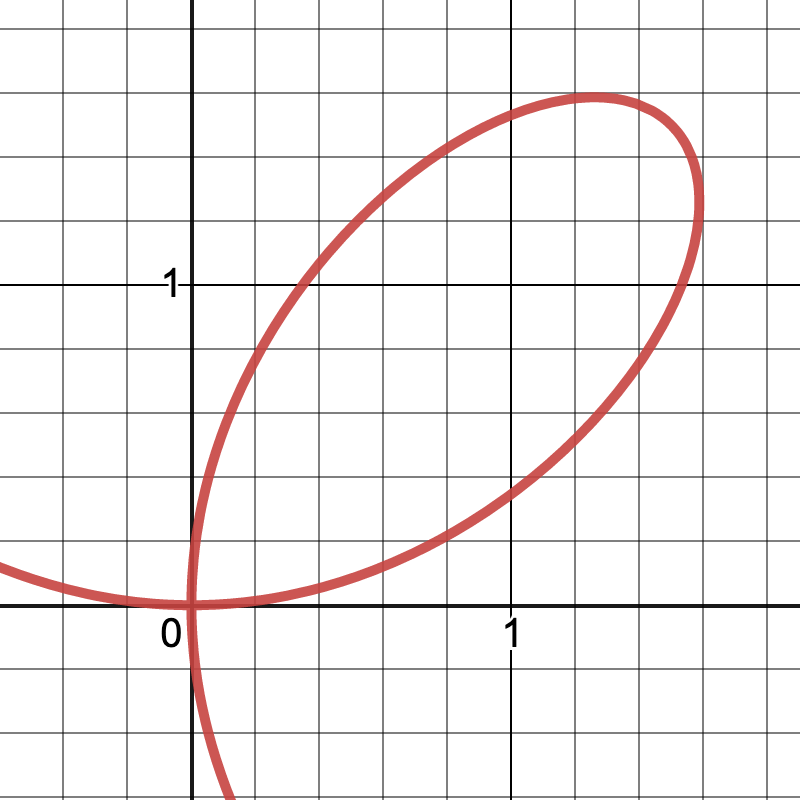
\includegraphics[scale=.25]{loop-3-8.png}

Tangent line to $y^3+x^3=3xy$ at $(3/2,3/2)$?

\end{multicols}

\vspace{1in}
 
 \item What is \quad \large{${\displaystyle{ \frac{d}{dx}\left[\:\left(f(x) \right)^3\:\right]}}$}\quad?\\
 
 \vfill
 
 \item Repeat question 2 above but with Leibniz notation assuming $y=y(x).$ Find $dy/dx$ for \large{${\displaystyle{\left(y \right)^3}}$}.\\
 
  \vfill
 
 \item Find \large{${\displaystyle{ \frac{d}{dx} \left[3xg(x) \right] }}$}.\\
 
  \vfill
 
 \item Find $dy/dx$ for \large{${\displaystyle{3xy}}$} assuming $y=y(x).$\\
 
  \vfill
  
  \newpage
  \item Find $dy/dx$ for each expression below.
  	\begin{enumerate}
	\item $x^2+y^3=\cos(x)+\sin(y) + \pi/2$
	\vfill
	\item $y \cos(x) +2x=(y+1)^2$
	\vfill
	\item $x+\tan(xy)=5$
	\vfill
	\end{enumerate}

\item For the equation $x^2+xy+y^2=9,$ 
	\begin{enumerate}
	\item Find the $x$ intercept(s).
	\vspace{.7in}
	\item Find the slope of the tangent lines at the $x$-intercepts.
	\vfill
	\item Write the equations of the tangent lines at the $x$-intercepts.
	\vspace{.5in}
	\end{enumerate} 
 


\end{enumerate}
\end{document}

